\documentclass[12pt,fleqn]{article}\usepackage{../../common}
\begin{document}
Materyel Mekaniği - 7

Burulma (Torsion)

Eksenel ve eksene dik yüklemelerden biraz daha çetrefil analiz gerektiren bir
yük uygulama şekli, bir çubuğun büküldüğü zaman ortaya çıkan burulma durumudur.
Burulma bir öğe momentlerle, ya da torklarla dönüşsel olarak yüklendiği zaman
ortaya çıkar [1, sf. 224].

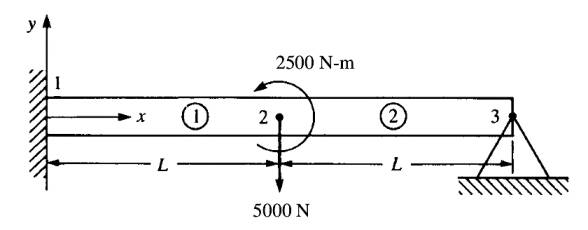
\includegraphics[width=10em]{phy_020_strs_06_01.jpg}

Mesela üstteki ilk resimde bir vidanın döndürülmesi görülüyor, bu durumda bir el
bir $T$ torku uygular. Bir arabanın tekerlek aksı, şaftı ya da gemilerin
pervanesine (propeller) dönüş ileten aks aynı davranışı sergiler.  Altta üçüncü
resimde görülen tork ilk nokta için $T_1 = P_1 d_1$ ile, ikincisi $T_2 = P_2
d_2$ ile hesaplanabilir.

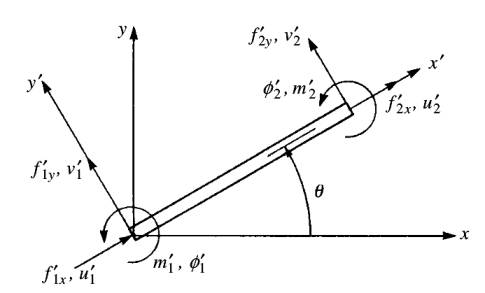
\includegraphics[width=15em]{phy_020_strs_06_02.jpg}

Burulma deformasyonunun mekaniğine biraz daha yakından bakalım. Bir çubuğu
$\phi(x)$ açısına gelecek şekilde büküyoruz, ve bu burulma bir $\gamma$ kaykılma
gerginliğine yol açıyor.

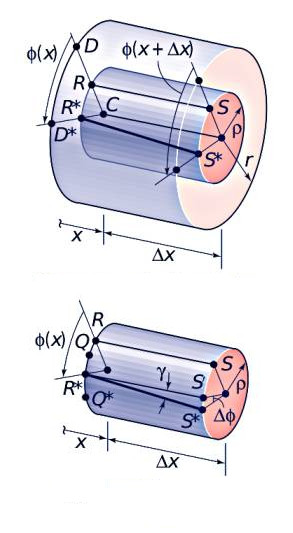
\includegraphics[width=10em]{phy_020_strs_06_03.jpg}

Üstteki ilk şekil çubuğun bir $x$ bağlamındaki bir parçasını gösteriyor,
altındaki ise o parçanın içindeki daha ufak yarıçaptaki bir parçasını [3, sf. 240]. 

$\gamma$ büyüklüğünü bulmak için üstteki resimde ikinci figure bakalım, $S^*$ ve
$S'$ arasındaki uzunluğu, $R^*$ ve $S'$ uzunluğuna bölersek (bu yapılabilir
çünkü ufak açılar sözkonusu ise tanjant hesabı aşağı yukarı açının kendisine
eşittir [2]) istenen sonucu bulabiliriz. Tabii $R^*S'$ uzunluğu $\Delta x$,
ve $S^*S'$ uzunluğu çember çevresinin ufak bir parçası, onu  $\rho \Delta \phi$
ile buluruz, bunları bir limit hesabı ile ifade edersek, ve $\Delta x \to 0$
iken

$$
\gamma = \lim_{\Delta x \to 0} \frac{S^*S'}{R^*S'} =
\lim_{\Delta x \to 0} \frac{\rho \Delta \phi}{\Delta x} =
\rho \frac{\ud \phi}{\ud x}
$$

O zaman eksenel yuvarlak olan bir birimin burumsal deformasyon için
gerginlik-yer değişim (strain-displacement) denklemi

$$
\gamma = \gamma(x,\rho) = \rho \frac{\ud \phi}{\ud x}
$$

$\phi$'in $x$'e göre türevi alınabildi çünkü formülü $x$'e bağlıdır, bunu
üstteki grafikte ilk figürde görüyoruz, $\phi(x)$ açısı $\phi(x+\Delta x)$
açısından farklı. Eğer $\phi$'yi formülsel olarak düşünsek herhalde $x$ arttıkça
ona lineer oranla artan bir açı büyüklüğü formülize edilebilirdi.

Kaykilma gerginligi ve stresi arasindaki iliskiyi daha once gorduk, burada da
bir Hooke Kanunu var,

$$
\tau = G \gamma
$$

$G$ sabiti kaykilma modulusu. 

Tüm bir yüzeydeki gerginlik için çubuğa yandan bakalım ve o tüm yan yüzeyde
etkili olan kaykılma stresini hesaplayalım. Ufak bir alan $\ud A$'ya
odaklanalım,

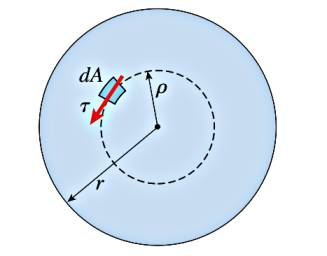
\includegraphics[width=10em]{phy_020_strs_06_04.jpg}

Gösterilen yüzeyde etkili olan kaykılma streslerinin dağılımı üstte işaretli. Bu
stresler sürekli olarak yüzeyde etkili oldukları için bir moment etkisi
yaratıyorlar, bu momentlerin toplamı çubuğa uygulanan torka eşit
olacaktır. Merkeze yarıçapsal $\rho$ uzaklığında bir $\ud A$ parçası düşünelim,
bu ufak bölgeye etki eden kaykılma stresi $\tau \ud A$'dir, ki $\tau$ yarıçap
$\rho$'da etkili olan kaykılma stresidir. Bu kuvvetin momenti kuvvet çarpı
merkeze olan uzaklık, bu örnekte uzaklık yine yarıçapın kendisi, o zaman ufak
moment $\ud M = \tau \rho \ud A$.

Ayrıca eğer verili bir yarıçap $r$ ve o yarıçapta etkili olan $\tau_{max}$
üzerinden formül yazmak istersek, dışarıdan içeri doğru giderken stresin
yarıçapa lineer bir şekilde değiştiğinden hareketle, yani

$$
\tau = \frac{\rho}{r} \tau_{max}
$$

olduğu için nihai entegral şöyle gösterilebilir,

$$
T = \int_A \ud M = \int_A \frac{\tau_{max}}{r} \rho^2 \ud A
$$

Bu entegral açısından $\tau_{max} / r$ sabit kabul edilip dışarı çekilebilir,

$$
T = \frac{\tau_{max}}{r} \int_A \rho^2 \ud A
$$

Geri kalan entegral $\int_A \rho^2 \ud A$ aslında her şekil için belli bir
formüle sahip olan kutupsal dönme direnci (polar moment of inertia), notasyonda
$I_P$ olarak geçer, bu örnekte bir çember şekli var, bu şekil için görülen
entegral

$$
I_P = \int_A \rho^2 \ud A
$$

şu değere sahiptir,

$$
I_P = \frac{\pi r^4}{2} 
$$


[devam edecek]

Kaynaklar

[1] Gere, {\em Mechanics of Materials}

[2] Bayramlı, {\em Normal Diferansiyel Denklemler, Trigonometri}

[3] Craig, {\em Mechanics of Materials}

\end{document}
